\documentclass[master]{subfiles}
\begin{document}
\title{\huge Nested Statistical Models for Temporal Affordance Learning in Vision-Based Autonomous Driving}
\author{
Eddie Zhou\thanks{Department of Operations Research and Financial Engineering, Princeton University, Princeton, NJ 08544, USA; e-mail: {\tt edzhou@princeton.edu}},~~
Chenyi Chen\thanks{Department of Operations Research and Financial Engineering, Princeton University, Princeton, NJ 08544, USA; e-mail: {\tt chenyi@princeton.edu}},~~
Han Liu\thanks{Department of Operations Research and Financial Engineering, Princeton University, Princeton, NJ 08544,USA; e-mail: {\tt hanliu@princeton.edu}}, ~ and
Alain Kornhauser\thanks{Department of Operations Research and Financial Engineering, Princeton University, Princeton, NJ 08544, USA; e-mail: {\tt alaink@princeton.edu}}
}
\date{}
\maketitle
\thispagestyle{empty}
% \vspace{-1em}
\begin{abstract}
Most current autonomous vehicle systems largely rely on Light Detection And Ranging (LIDAR), but there is much room for development in purely vision-based systems.  Recently, a DeepDriving paradigm of learning affordance indicators from input images was suggested.  We extend this model by analyzing the temporal and sequential nature of the input images.  To do so, we apply convolutional feature extraction and examine three problems: the usefulness of history, the lag selection problem, and the viability of complex models with history.  We train recurrent, or ``nested'' statistical models of varying complexity, and our results demonstrate that the sequential aspect of this problem is highly important and appropriate for such recurrent statistical models.
\end{abstract}
\vspace{1em}
\noindent {\bf Keywords:} convolutional neural network; nested models; recurrent; autonomous driving; image recognition, regression, multivariate adaptive regressive splines.
\section{Introduction}\label{intro}
Predictive statistical models are formulated, trained, and used in a variety of applications, from spam filtering and recommender systems to outlier detection and image recognition.  One such application that has not been thoroughly explored from a statistical standpoint is autonomous driving.  Within this application, vision-based approaches typically adopt one of two paradigms: mediated perception (parsing an entire scene to make a driving decision), or behavior reflex (mapping an input image to a driving action).  For a more thorough survey of these paradigms, see \cite{deepdriving}.  In their work, \cite{deepdriving} also propose an intermediate, ``DeepDriving'' paradigm that strikes a balance between the two.  In their work, image representations are mapped onto a small set of ``affordance indicators''.  These values are effectively a distillation of the driving conditions -- they include values such as distances to lane markings and other vehicles, road angles, and others.  A simple logic controller can then take the affordance indicator values and translate them into operation of the vehicle accordingly.\par
DeepDriving still relies on a model that maps an input vector $\mathbf{x} \in \mathbb{R}^n$ and outputs a vector of continuous values $\mathbf{y} \in \mathbb{R}^m$, which points to the task of statistical regression.  While the problem of image classification is largely solved with the advancement of deep learning methods (namely, deep convolutional neural networks, or CNNs), our image regression problem is slightly different.  The more important aspect of the data at hand is its temporal and sequential nature -- in a real setting, images captured by the autonomous vehicle would be processed one after another.  Then, at a realistic granularity, previous images should affect the current driving decisions.  \cite{deepdriving} relied largely on the widely-used CNNs to map input images to the aforementioned affordance indicators.  While powerful, CNNs do not take advantage of any temporal features in the data, as recurrent neural networks do.\par
Our goal for this paper, however, is not to replicate the work of \cite{deepdriving} and substitute in recurrent neural networks.  Instead, we look to apply rigorous statistical analysis to investigate the role of history in predicting affordance indicator values, and subsequently understand the viability of this history in both linear and nonlinear models.  We characterize our approach in three problems: the first is to rigorously determine whether past history is predictively useful at all.  To do so, we build simple linear models and use p-value analysis for the relevant coefficients.  Second, we look to solve the lag order selection problem, which asks the optimal number of past data to include for predictive performance optimization.  We approach this second problem through model selection using stacked evaluation metrics.  Finally, we examine the predictive viability of nonlinear models operating on historical, lag order selected data, hoping to show that the usefulness of history extends to more complex models.\par
\subsection{Related Works}
This paper largely builds off of the work of \cite{deepdriving} in validating the DeepDriving, or direct perception, paradigm.  As mentioned in Section \ref{intro}, they train a convolutional neural network with data extracted from the TORCS driving video game.  The inputs are convoluted image features, while the output is a set of 14 continuous values: the affordance indicators passed to the logic controller.  The output data is available via extraction from the game engine, as are the input images (which are passed through a CNN for feature extraction).  Note that in our work, we also use the dataset presented in their work.  Doing so allows us to investigate the temporal nature within the exact same assumptions.\par
We also make use of work done by \cite{aic_bic1}, \cite{aic_bic2}, and \cite{liew} in the usage of model selection metrics with respect to the lag order selection problem.  The convolutional neural network used in our feature extraction also relies on the standard structure set forth by \cite{lenet}.  Our nonlinear work is advanced by the seminal paper on MARS, by \cite{mars}, as well as the fast heuristic added in \cite{fastmars}.
\subsection{Paper Organization}
The rest of this paper is organized as follows.  Section \ref{sec:data_tools} introduces details of the dataset, explains the feature extraction process, and gives a brief summary of the software used for model fitting.  In Sections \ref{sec:single_history}, \ref{sec:lag_order}, \ref{sec:nonlinear}, we refine the three problems presented: deciding whether history is predictively significant, rigorously determining the lag order, and examining the viability of more complex, nonlinear models.  Section \ref{sec:results} provides numerical and graphical results for the three problems, and section \ref{sec:discussion} contains discussion thereof.
\newpage
\section{Data Wrangling and Tools}\label{sec:data_tools}
\subsection{Data Pipeline}
The TORCS dataset exists as a leveldb, a data storage format also developed and used by Google.  We use Python's \lstinline{leveldb} module to connect and read from the images and values stored within it.  We also need to use Python's \lstinline{Caffe} interface to access the \lstinline{Datum} objects stored within the database.  Iterating through the leveldb, we fill \lstinline{numpy} arrays of dimension 10000 x 3 x 210 x 280, and use \lstinline{hickle} to save the batched arrays.  The dimensions are explained as follows: the data are 3 color channel images, each image is of resolution 210 x 280, and 10000 is the largest even data size that fits in memory.  Dividing the data into chunks of 10000 is also suitable for the batched aspect of stochastic gradient descent used later.  Finally, we also extract the 14 affordance indicator labels (true values) for each of the 484815 images from the leveldb, and store the resulting 484815 x 14 output matrix separately.
\subsection{Feature Extraction}
We first train a convolutional neural network with LeNet architecture as first proposed by \cite{lenet} for the purpose of feature extraction.  We implement the network with \lstinline{nolearn} by \cite{nolearn}, a software library that allows for flexible neural network training in the format of the widely-used \lstinline{scikit-learn} Python library.  \lstinline{nolearn} wraps \lstinline{Lasagne} by \cite{lasagne}, which is, in turn, an abstraction of \lstinline{Theano}, by \cite{theano}.\par
For our feature extraction network, each response variable is scaled to [0, 1].  For a response $y_{ij}$, representing the $i$th affordance indicator of the $j$th data point, we scale using the minimum and maximum values over all $j$, holding $i$ constant:
\begin{align*}
y_{ij}^{(s)} = \frac{y_{ij} - \min_jy_{ij}}{\max_jy_{ij} - \min_jy_{ij}}
\end{align*}
Output scaling is done during this process in order to facilitate convergence.  Data is loaded and subsequently passed through the model in the aforementioned batches of 10000.  We extract the features as the last hidden layer, which has 500 nodes.  Therefore, our final training matrix $\mathbf{X}^{(CNN)}$ is 484815 x 500, where one datum, or image, is represented by 500 convoluted image features.
\subsection{Training and Testing}
In Section \ref{sec:single_history}, we use the Ordinary Least Squares implementation of the \lstinline{statsmodels} package in Python, by \cite{statsmodels}, for our model training and evaluation.  Then, due to an increased need for computational efficiency, in Section \ref{sec:lag_order} and part of Section \ref{sec:nonlinear}, we use the implementation of stochastic gradient descent within \lstinline{scikit-learn}, a popular Python library for machine learning developed by \cite{scikit-learn}.  Finally, for one of our nonlinear models in \ref{sec:nonlinear} we use an implementation of Multivariate Adaptive Regression Splines, within \lstinline{py-earth}, by \cite{py-earth}.
\clearpage
\section{Single History Inclusion}\label{sec:single_history}
We perform ordinary least squares regression with two model structures: one with the time $t$ convoluted image features as input, and one with both the time $t$ and time $t - 1$ convoluted image features as input.  For this analysis, we refer to the $t$ structure as ``Model 1'', indicated by $\hat{\mathbf{y}}_t$,  and the $t, t-1$ structure as ``Model 2'', indicated by $\tilde{\mathbf{y}}_{t, t-1}$.  For both structures, we train 14 separate models, each predicting a single affordance indicator, or response variable.  The two models can be expressed in least squares regression modelling as the following:
\begin{align*}
\hat{\mathbf{y}}_t^{(a_1)} &= \bm{\beta}^{(a_1)}\mathbf{X_t} + \bm{\epsilon}\\
\tilde{\mathbf{y}}_{t, t-1}^{(a_1)} &= \bm{\beta_t}^{(a_1)}\mathbf{X_t} + \bm{\beta_{t-1}}^{(a_1)}\mathbf{X_{t-1}} + \bm{\epsilon}\\
\hat{\mathbf{y}}_t^{(a_2)} &= \bm{\beta}^{(a_2)}\mathbf{X_t} + \bm{\epsilon}\\
\tilde{\mathbf{y}}_{t, t-1}^{(a_2)} &= \bm{\beta_t}^{(a_2)}\mathbf{X_t} + \bm{\beta_{t-1}}^{(a_2)}\mathbf{X_{t-1}} + \bm{\epsilon}\\
&.\\&.\\&.\\
\hat{\mathbf{y}}_t^{(a_{14})} &= \bm{\beta}^{(a_{14})}\mathbf{X_t} + \bm{\epsilon}\\
\tilde{\mathbf{y}}_{t, t-1}^{(a_{14})} &= \bm{\beta_t}^{(a_{14})}\mathbf{X_t} + \bm{\beta_{t-1}}^{(a_{14})}\mathbf{X_{t-1}} + \bm{\epsilon}\\
\end{align*}
After fitting these 28 models with OLS, we will analyze the p-values for each coefficient, across all affordance indicators (500 x 14 for model 1, and 1000 x 14 for model 2).  As a brief reminder on the elementary statistics of least-squares coefficients, each coefficient's p-value is the result of a $t$-test with the null hypothesis that the coefficient itself is zero.  Therefore, finding significantly low values for the p-values corresponding to the coefficients of the past time step will demonstrate that history has predictive value within this model.
\section{Lag Order Selection}\label{sec:lag_order}
Assuming predictive significance of past history, the next step is to decide exactly how much history is relevant -- in other words, to examine the lag order selection problem.  To do this, we again fit a series of simple linear models -- now, however, each model corresponds to including varying amounts of history, from only the most recent image to the previous 12 images.  We wrangle the 484815 x 500 $\mathbf{X}^{(CNN)}$ matrix into 12 more matrices, each corresponding to using one more previous time step.  These are of dimension 484814 x 1000, 484813 x 1500, etc.  Notice that we lose one more data point from the beginning of the temporal sequence with each time inclusion.  We see this by noting that our first data point has no $t-1$ image to concatenate for one time step inclusion, our second data point has no $t-2$ image to concatenate for two time step inclusions, and so on.  We only lose 12 data from the beginning of the sequence, however, which is negligible with respect to the magnitude of our entire dataset.\par
Naive OLS matrix inversion is no longer computationally viable for these larger matrices, so we use the classical method of stochastic gradient descent (SGD), with squared loss and an L2, or ridge, penalty.  Due to the high dimensionality, we also use a large penalty multiplier to push coefficients closer to 0, as well as a higher number of training epochs.\par
We can apply model selection between the 12 structures using three different evaluation metrics.  The first two, Akaike and Bayesian information criterion (AIC and BIC, respectively), are classical relative measures for statistical models based on empirical likelihood.  As likelihood-based methods, they can be computed entirely from the result of model training, eliminating the need to hold out a test set.  For both criteria, lower values point to better models.  Because we have 14 affordance indicators, however, we must compute ``stacked'' versions of the AIC and BIC.  These are versions of the standard AIC and BIC that aggregate across each affordance indicator.  The time inclusion can be seen as a model structure, so we want to compare these metrics for each time inclusion, not across the response variables.  Standard and stacked IC formulas, as a function of the linear coefficients $\boldsymbol{\beta}$, are given as follows:
\begin{align*}
&\text{AIC}(\boldsymbol\beta) = 2k - 2\log(\hat{L})\\
&\text{BIC}(\boldsymbol\beta) = k\log N - 2\log(\hat{L})\\
&\text{AIC}^{(t-s)}(\boldsymbol\beta^{(t-0)}, \boldsymbol\beta^{(t-1)}, ..., \boldsymbol\beta^{(t-s)}) = 2\sum_{a=1}^{14}k_a - 2\sum_{a=1}^{14}\log(\hat{L}_a)\\
&\text{BIC}^{(t-s)}(\boldsymbol\beta^{(t-0)}, \boldsymbol\beta^{(t-1)}, ..., \boldsymbol\beta^{(t-s)}) = \sum_{a=1}^{14}k_a\log N_a - 2\sum_{a=1}^{14}\log(\hat{L}_a)
\end{align*}
where $k$ is the model degree of freedom (number of non-zero predictor coefficients), and the log-likelihood is calculated as follows:
\begin{align*}
\log(\hat{L}) &= -\frac{N}{2}\log(2\pi\hat{\sigma}^2) - \frac{SSR}{2\hat{\sigma}^2}\\
SSR &= \sum_{i=1}^N(y_i - \hat{y}_i)^2\\
\hat{\sigma}^2 &= \frac{SSR}{N}
\end{align*}
Our third model selection metric is evaluation-based, and requires withholding a test set.  The RMSE, or root-mean-square-error, is frequently used in statistics and machine learning for evaluating predictive performance.  We apply an 80/20 split to our dataset, using 80\% of the data to train 14 models for each time inclusion structure.  Then, we can evaluate the models on the remaining 20\% of the data by aggregating RMSE across all 14 affordance indicators for each time step:
\begin{align*}
&RMSE(\boldsymbol\beta) = \sqrt{\frac{\sum_{i=1}^N(y_i - \hat{y}_i)^2}{N}}\\
&RMSE^{(t-s)}(\boldsymbol\beta^{(t-0)}, \boldsymbol\beta^{(t-1)}, ..., \boldsymbol\beta^{(t-s)}) = \sqrt{\frac{\sum_{a=1}^{14}\sum_{i=1}^N(y_{i, a} - \hat{y}_{i, a})^2}{\sum_{a=1}^{14}N_a}}
\end{align*}
\clearpage
\section{Nonlinear Models}\label{sec:nonlinear}
If we solve the lag order selection problem, we would like to examine if including history provides better predictive power in models beyond simple linear models.  We therefore choose to examine two nonlinear models with our selected lag order, and evaluate them on prediction metrics given above to analyze their viability.  These two models are chosen for their simplicity and because they exist as simple conceptual extensions of linear models.
\subsection{Basis Expansion}
The first nonlinear model we explore is a simple basis expansion model.  There is an abundance of basis expansions that are viable, with infinite polynomial operations.  Because we are not concerned with feature-feature interaction and we wish to retain computational feasibility, however, we simply add a polynomial basis expansion for each response variable up to the third power.
\begin{align*}
\mathbf{x} &= [x_1, x_2, ..., x_k]\\
\mathbf{x}^{(expand)} &= [x_1, x_1^2, x_1^3, x_2, x_2^2, x_2^3, ..., x_k, x_k^2, x_k^3]
\end{align*}
Depending on the selected lag order $s$, the data will then have a new dimension of $1500s$, as each additional lag order provides another 500 dimensions, and the basis expansion provides another factor of 3.  After expanding the basis, it becomes a matter of fitting another simple linear model with stochastic gradient descent to the new, expanded data and evaluating it.\par
\subsection{Multivariate Adaptive Regressive Splines}
The next nonlinear framework to explore is multivariate adaptive regressive splines (MARS), introduced by \cite{mars}.  This process is a more complex nonlinear method than simply extending the basis and fitting a linear model.  As a non-parametric regression, MARS models non-linearities through basis functions composed of a constant, a hinge function, or a product of multiple hinge functions.  MARS training is done with a greedy forward pass that adds basis functions that give maximal reduction in SSR, followed by a backwards pass that prunes the model using generalized cross validation, which can be seen as a form of regularization.\par
Due to the expensive nature of the continual forward and backward passes, there are various heuristics to speed up the model.  The first heuristic, proposed by the original author of MARS in \cite{fastmars}, limits the maximum number of parent terms considered at each step of the forward pass.  It does so by cutting off the priority queue ranking of parent functions at some parameter $K$.\par
This fast heuristic is usually available in implementations of MARS, and is controlled by varying the \lstinline{fast_K} parameter.  In general, lower values of the parameter decrease the training time (decreasing the number of parent terms considered), but at the expense of the quality of the model.  Higher values generally result in longer training times and stronger models, but random variation makes this rule general, rather than rigid, as per \cite{earth}.\par
\section{Results}\label{sec:results}
\subsection{History Inclusion}
The first model simply predicts the response values as a linear function of the current time step's image features.  As expected, we see low p-values for a significant number of the 500 features.  For almost every affordance indicator, the median p-value (across all 500 coefficients) is less than 0.05, demonstrating that over half of the convoluted image features in each of the 14 individual models are significant at a 5\% confidence level.  Table \ref{table:p1} shows the distributions of these 500 p-values in the form of summary statistics for each affordance indicator.
\begin{table}[H]
\centering
\caption{p-value summary for Model 1  $\bm{\beta}$ coefficients.}
\begin{tabular}{@{}lllllll@{}}
\toprule
    & Min.       & 1st Qu.   & Median    & Mean   & 3rd Qu. & Max.   \\ \midrule
$a1$  & 0          & 1.541e-31 & 1.142e-05 & 0.2229 & 0.6058  & 0.9716 \\
$a2$  & 0          & 1.697e-05 & 0.1004    & 0.2926 & 0.6946  & 0.9889 \\
$a3$  & 7.275e-218 & 1.569e-12 & 0.02273   & 0.294  & 0.7537  & 0.9964 \\
$a4$  & 0          & 4.727e-10 & 0.04213   & 0.2813 & 0.6944  & 0.9874 \\
$a5$  & 0          & 1.655e-14 & 0.009673  & 0.1359 & 0.1436  & 0.9978 \\
$a6$  & 0          & 2.698e-13 & 0.007431  & 0.2    & 0.3722  & 0.9859 \\
$a7$  & 0          & 3.849e-14 & 0.003059  & 0.1093 & 0.05035 & 0.9935 \\
$a8$  & 0          & 3.372e-09 & 0.001924  & 0.1226 & 0.07164 & 0.9831 \\
$a9$  & 0          & 1.47e-06  & 0.06613   & 0.2064 & 0.3358  & 0.9971 \\
$a10$ & 0          & 9.744e-09 & 0.01287   & 0.1966 & 0.415   & 0.9866 \\
$a11$ & 0          & 4.802e-09 & 0.007885  & 0.1157 & 0.07668 & 0.9934 \\
$a12$ & 0          & 1.234e-10 & 0.005826  & 0.1    & 0.03029 & 0.9981 \\
$a13$ & 6.051e-291 & 2.937e-09 & 0.0194    & 0.2836 & 0.7434  & 0.9874 \\
$a14$ & 0          & 2.422e-07 & 0.00165   & 0.1384 & 0.1424  & 0.9953 \\ \bottomrule
\end{tabular}
\label{table:p1}
\end{table}
\vspace{1em}
In the second model, we input both the 500 convoluted image features of the current time step, as well as the 500 convoluted image features of the previous time step, for a total of 1000 features.  In Tables \ref{table:p2} and \ref{table:p3}, we see that the p-value distribution for the 500 $\bm{\beta_t}$ coefficients in Model 2 is larger than the corresponding distribution of 500 p-values in Model 1.  This is intuitive, though, given the addition of 500 new features not included in Model 1 and increased model size.  More features inherently means that a sufficiently parsimonious model will regard fewer features as important, and the p-value distribution will be shifted to the right compared to a smaller model.  Moreover, the p-values for the $\bm{\beta_{t-1}}$ coefficients are overwhelmingly significant, which answers our question of interest.  It is clear that the features from the previous time step are significant in predicting affordance indicators for the current time step -- we include a graphical representation of the distribution of the $\bm{\beta_{t-1}}$ p-values for further confirmation. 
\begin{table}[H]
\vspace{5em}
\centering
\caption{p-value summary for Model 2 $\bm{\beta_t}$ coefficients.}
\begin{tabular}{@{}lllllll@{}}
\toprule
    & Min.       & 1st Qu.   & Median   & Mean   & 3rd Qu. & Max.   \\ \midrule
$a1$  & 1.868e-287 & 2.627e-09 & 0.02677  & 0.2161 & 0.4138  & 0.9925 \\
$a2$  & 3.211e-106 & 0.009934  & 0.3882   & 0.4276 & 0.862   & 0.9988 \\
$a3$  & 1.271e-74  & 0.0003873 & 0.226    & 0.396  & 0.9093  & 0.9999 \\
$a4$  & 8.369e-128 & 0.0004557 & 0.2257   & 0.3932 & 0.8869  & 1      \\
$a5$  & 1.361e-81  & 0.0003228 & 0.04829  & 0.1531 & 0.1317  & 0.9982 \\
$a6$  & 1.681e-85  & 5.213e-05 & 0.1444   & 0.1871 & 0.2097  & 0.9908 \\
$a7$  & 4.051e-105 & 8.328e-05 & 0.01527  & 0.1447 & 0.1641  & 1      \\
$a8$  & 1.943e-135 & 0.0001521 & 0.0088   & 0.1519 & 0.1899  & 0.9959 \\
$a9$  & 4.69e-78   & 0.009723  & 0.1822   & 0.2368 & 0.3035  & 0.9915 \\
$a10$ & 8.137e-100 & 0.001327  & 0.1711   & 0.2912 & 0.5374  & 0.9975 \\
$a11$ & 3.133e-100 & 0.0004654 & 0.009569 & 0.1409 & 0.1303  & 0.9973 \\
$a12$ & 1.215e-151 & 0.0001589 & 0.008946 & 0.1281 & 0.1532  & 0.9921 \\
$a13$ & 6.864e-72  & 0.00198   & 0.2783   & 0.3594 & 0.7223  & 0.9886 \\
$a14$ & 1.091e-116 & 0.0005832 & 0.00637  & 0.1561 & 0.2204  & 0.9986 \\ \bottomrule
\end{tabular}
\label{table:p2}
\end{table}
\begin{table}[H]
\centering
\caption{p-value summary for Model 2 $\bm{\beta_{t-1}}$ coefficients.}
\begin{tabular}{@{}lllllll@{}}
\toprule
    & Min.       & 1st Qu.   & Median   & Mean   & 3rd Qu. & Max.   \\ \midrule
$a1$  & 0          & 4.004e-14 & 0.001513 & 0.1808 & 0.401   & 0.9868 \\
$a2$  & 0          & 3.374e-05 & 0.0695   & 0.2896 & 0.6123  & 0.9954 \\
$a3$  & 1.875e-123 & 6.232e-08 & 0.04029  & 0.292  & 0.6005  & 0.9992 \\
$a4$  & 2.921e-150 & 4.874e-07 & 0.05511  & 0.2675 & 0.5239  & 0.9988 \\
$a5$  & 2.609e-193 & 3.417e-08 & 0.03431  & 0.1649 & 0.2446  & 0.9952 \\
$a6$  & 3.009e-183 & 1.626e-07 & 0.03167  & 0.1852 & 0.2335  & 0.9921 \\
$a7$  & 4.245e-292 & 1.435e-08 & 0.006297 & 0.1501 & 0.1567  & 0.9934 \\
$a8$  & 0          & 1.514e-06 & 0.005839 & 0.1487 & 0.1798  & 0.9977 \\
$a9$  & 0          & 1.412e-05 & 0.05789  & 0.2005 & 0.2799  & 0.9996 \\
$a10$ & 5.842e-206 & 4.892e-05 & 0.06788  & 0.2259 & 0.4497  & 0.9921 \\
$a11$ & 2.047e-131 & 1.548e-05 & 0.01567  & 0.1896 & 0.2996  & 0.9976 \\
$a12$ & 6.702e-140 & 9.075e-06 & 0.009431 & 0.1585 & 0.1948  & 0.9923 \\
$a13$ & 3.324e-69  & 0.0001888 & 0.07977  & 0.2762 & 0.6316  & 0.9882 \\
$a14$ & 3.431e-107 & 0.0001382 & 0.02132  & 0.1873 & 0.2827  & 0.9939 \\ \bottomrule
\end{tabular}
\label{table:p3}
\end{table}
\begin{figure}[H]
\vspace{6em}
\centering
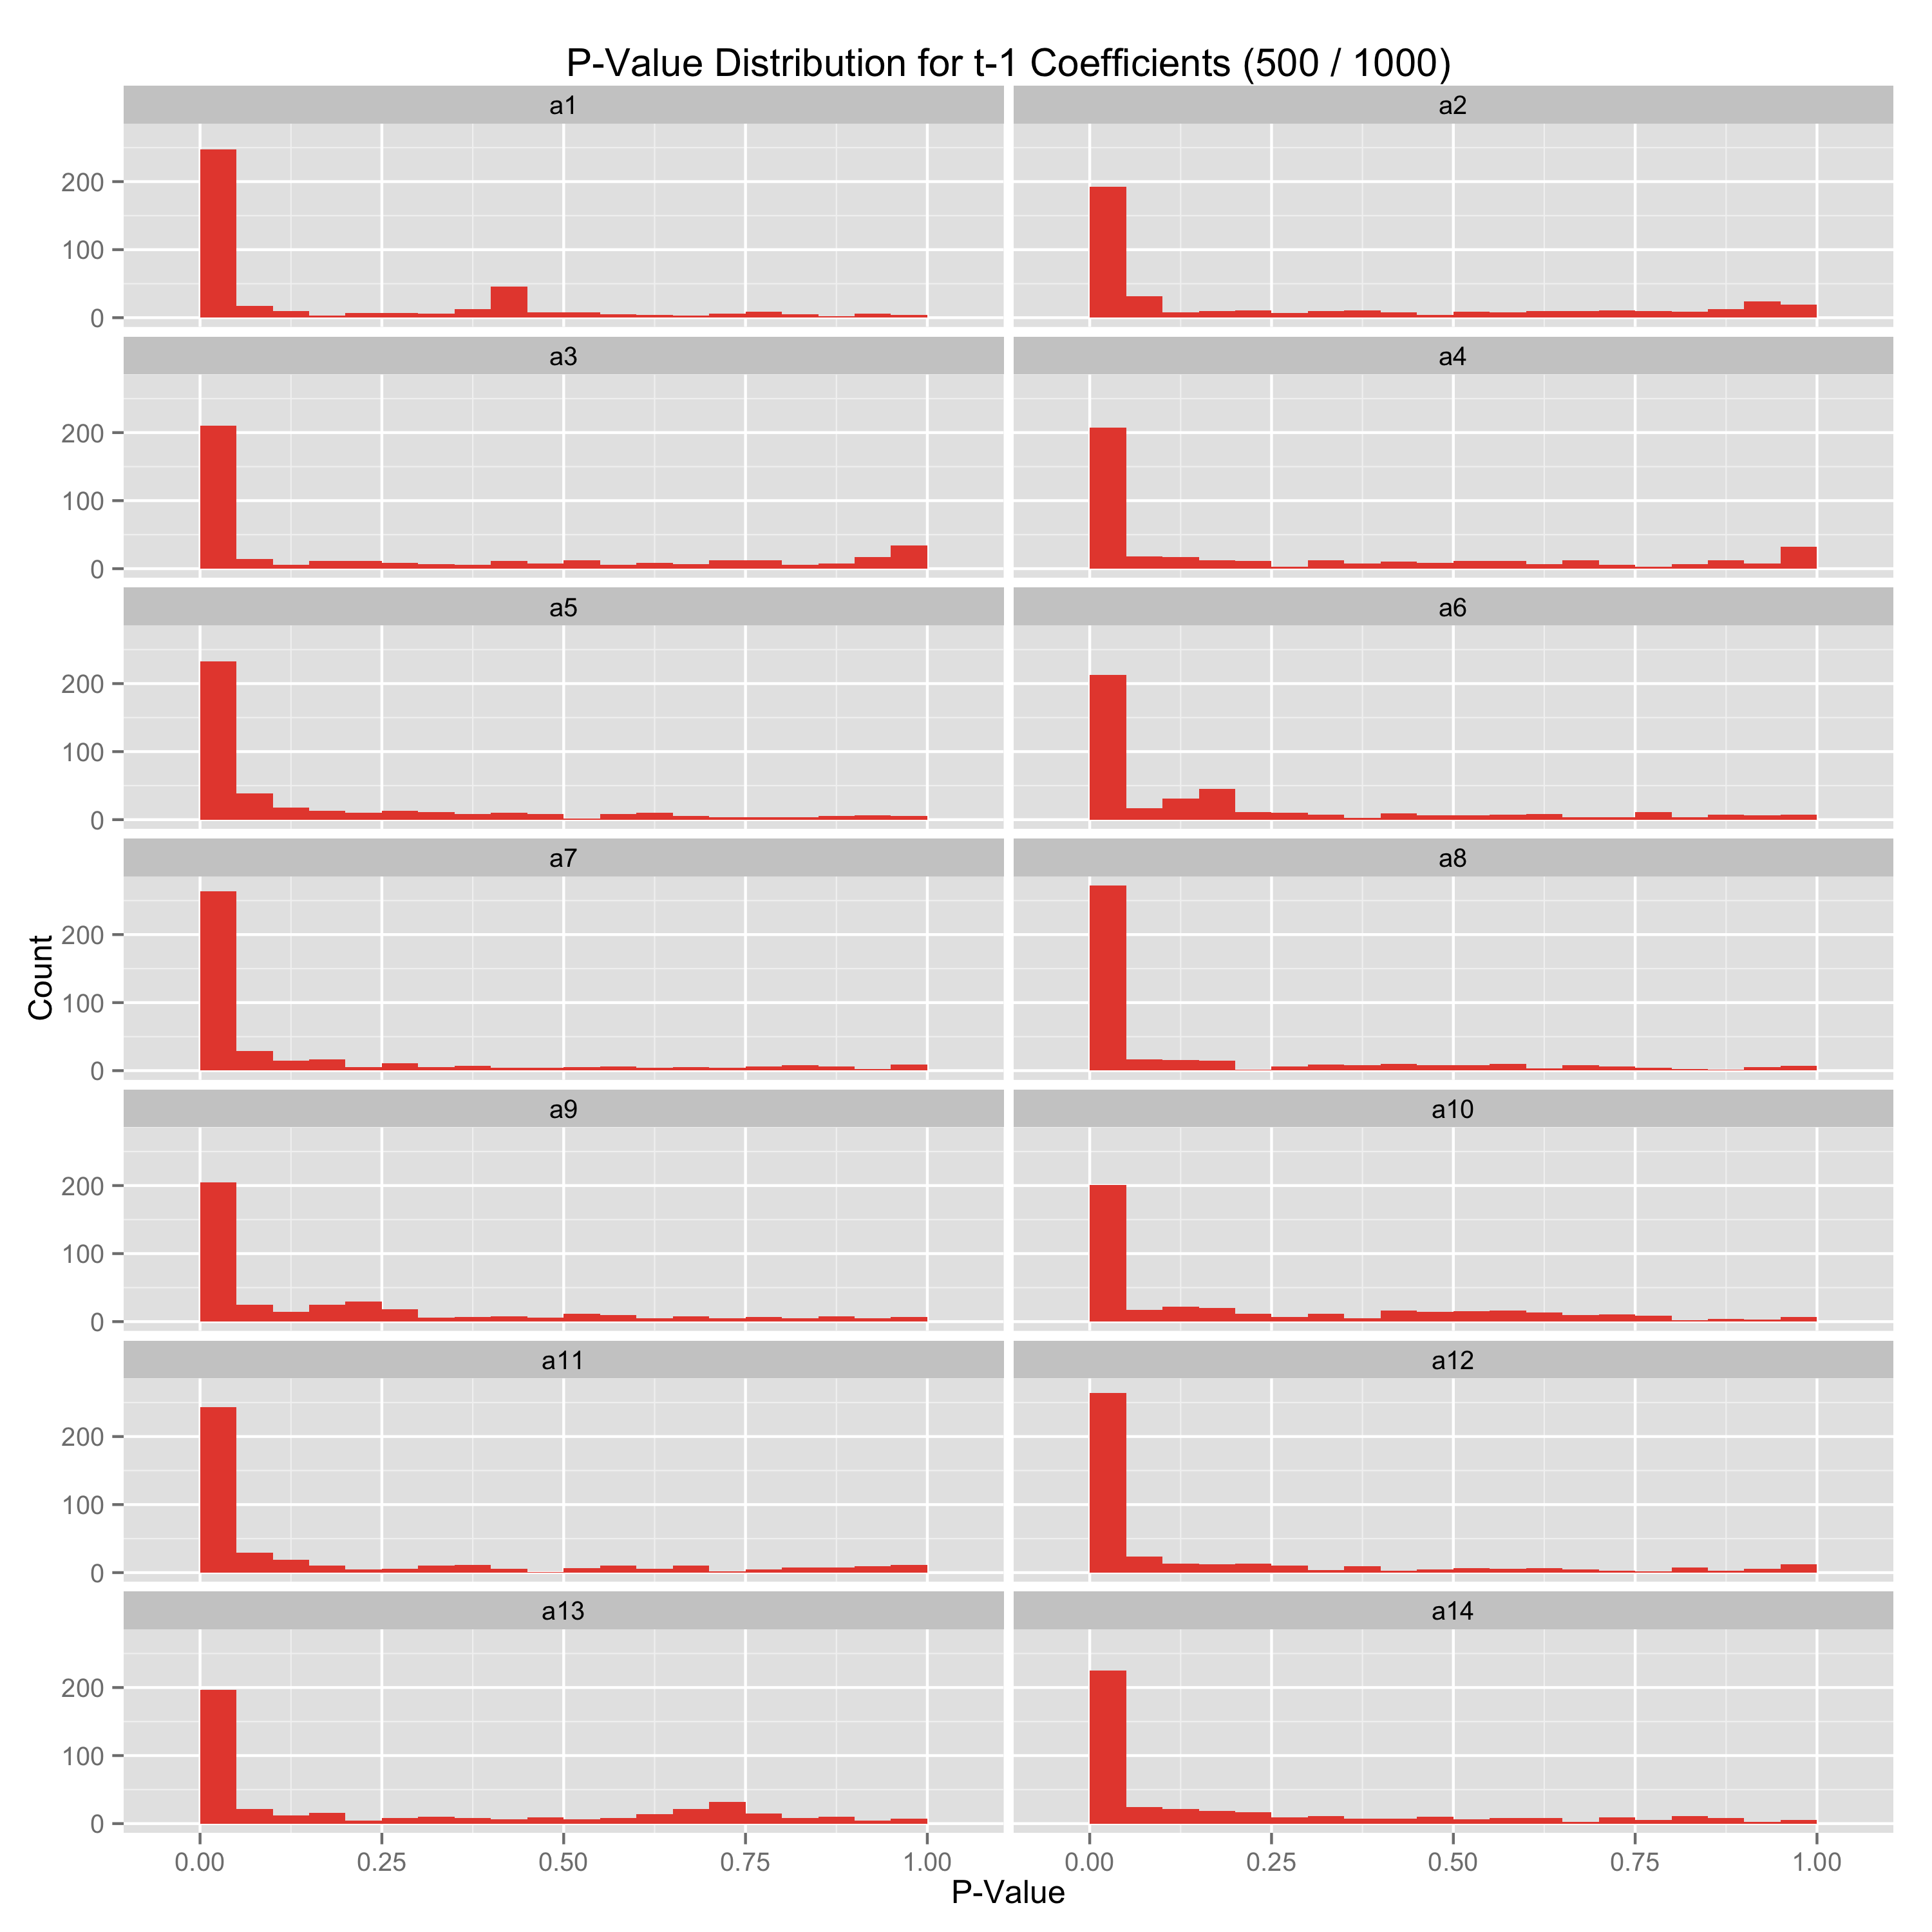
\includegraphics[width=155mm]{figs/t1_tminus1_pvals.png}
\caption{The distributions of the 500 $t-1$ step p-values in our Model 2 structure.  For each of the 14 models, each corresponding to a response variable, these histograms show that nearly half of the p-values fall in the 0.05 bucket.  This indicates that past history, in the form of the previous time step's convolute image features, is statistically significant for prediction within the model.}
\label{fig:p_dist}
\end{figure}
\newpage
\subsection{Lag Order Selection}\label{sec:lag-order-results}
As described in Section \ref{sec:lag_order}, we calculate stacked information criterion and aggregate RMSE values for each additional inclusion of history.  The model selection criteria are plotted in Figures \ref{fig:stacked_ic} and \ref{fig:rmse}, along with dashed lines representing LOESS-smoothing.
\begin{figure}[H]
\centering
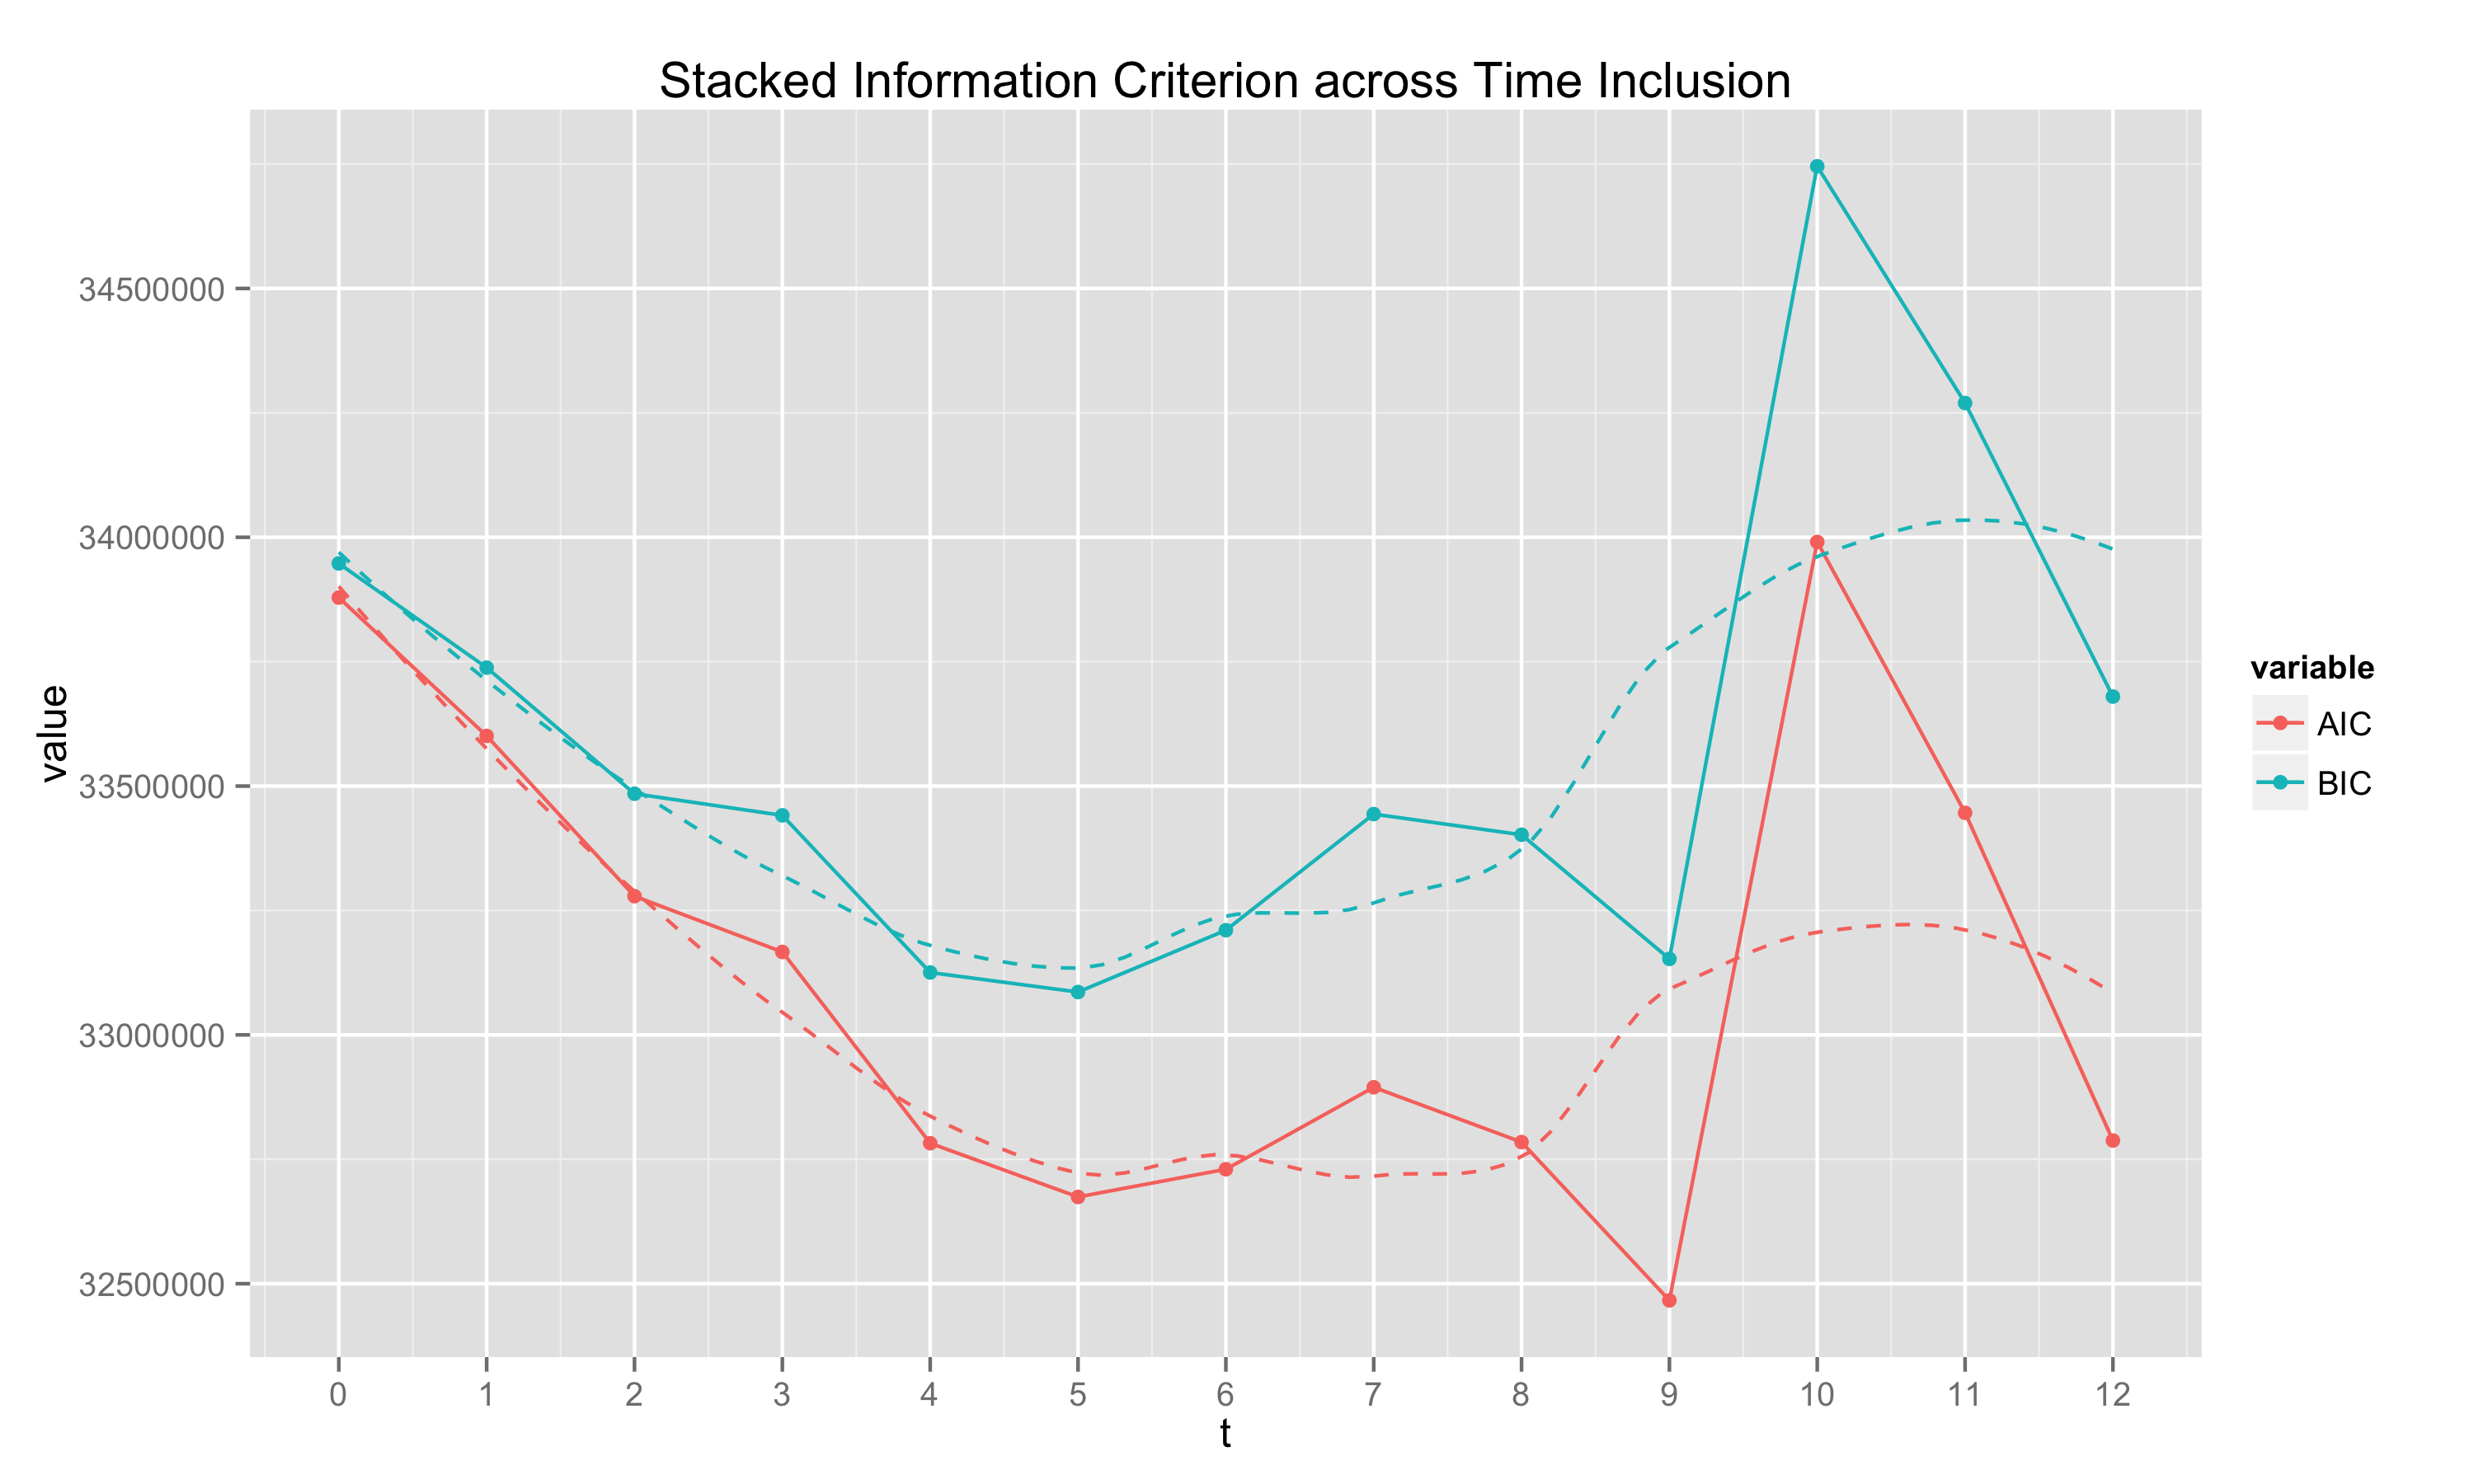
\includegraphics[width=150mm]{figs/sgd_stacked_ic.png}
\caption{Stacked AIC and BIC for each additional time step inclusion.}
\label{fig:stacked_ic}
\end{figure}
\begin{figure}[H]
\centering
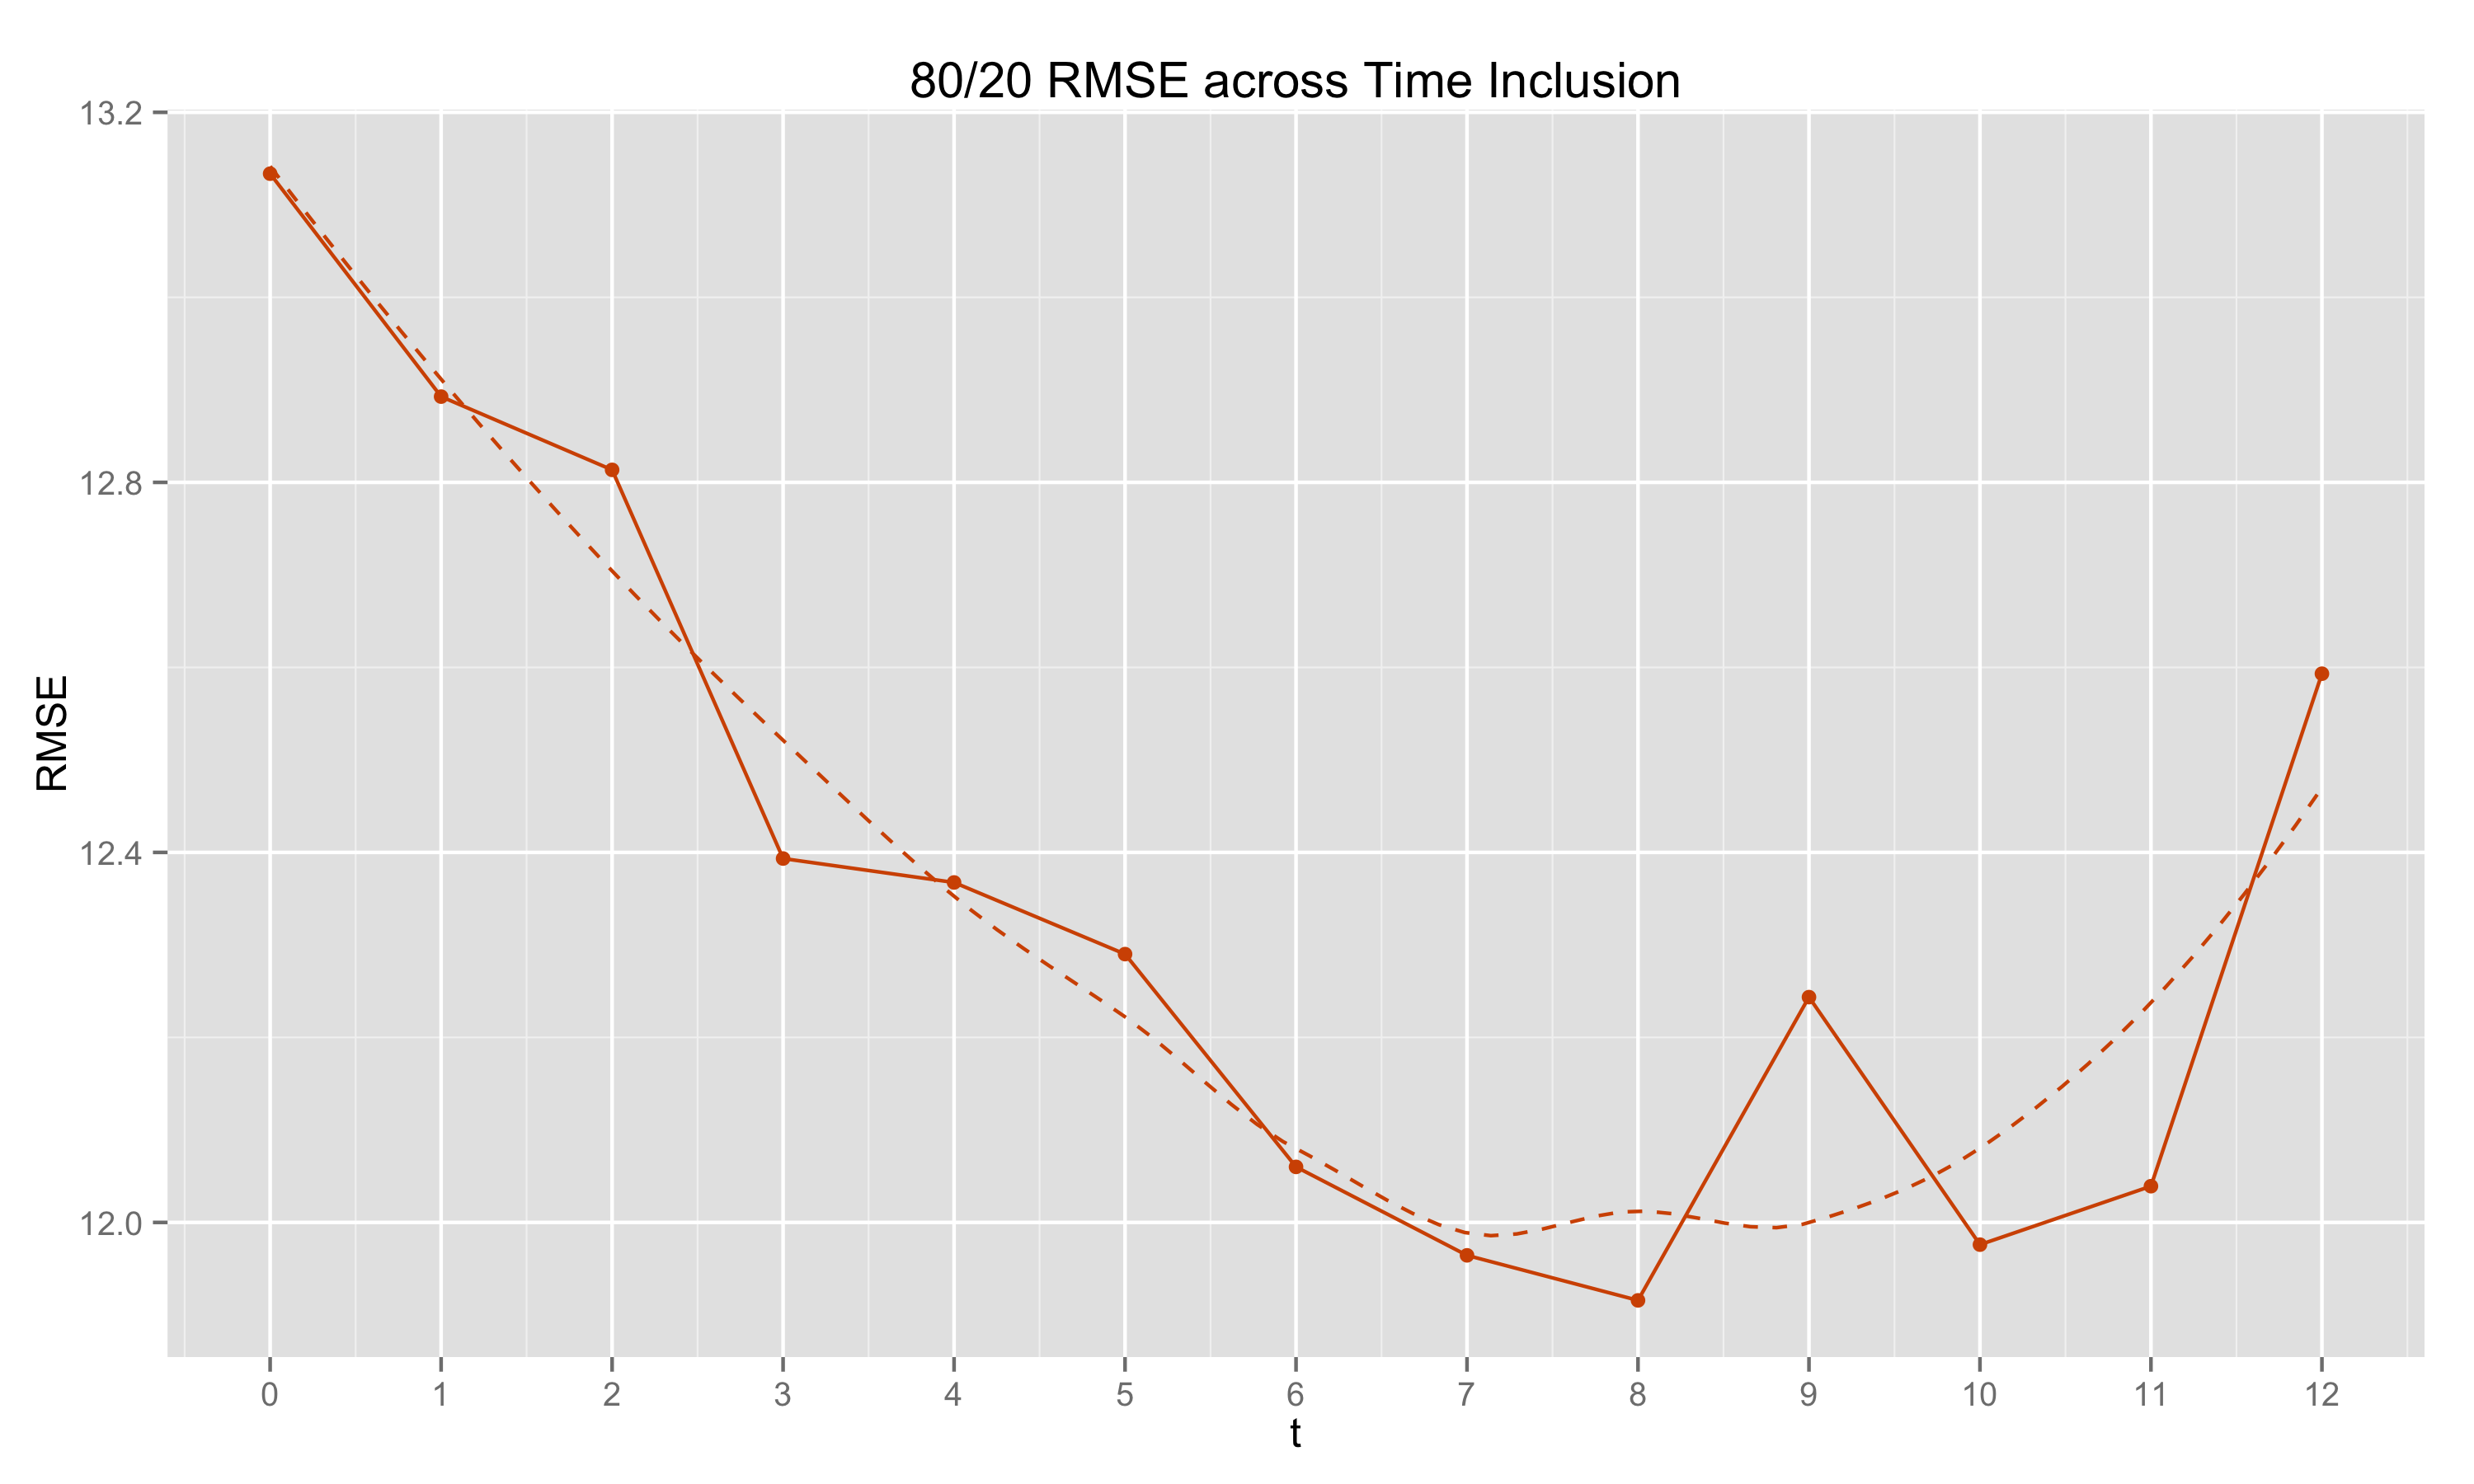
\includegraphics[width=140mm]{figs/sgd_rmse.png}
\caption{Aggregated RMSE for each additional time step inclusion.}
\label{fig:rmse}
\end{figure}
In the stacked information criterion plot, we see a steady decrease of both AIC and BIC as we include more history, until we get to $t-5$.  When we include the past 6 convoluted features, though, both of the information criterion begin to rise again, and we see much more noise.  In the aggregated RMSE plot, we see a similarly convex curve that decreases until around $t-7$, and then begins rising (again, with more noise on the ascent).  It is clear that there is a decrease, followed by a noisy increase, and that the smallest value lies somewhere in the aforementioned range.\par
The implementation of the stacked IC and the nature of RMSE dictates that smaller values point to better models.  In using these metrics, we note that BIC seeks the ``true'' model, whereas AIC tries to select the model that most adequately describes an unknown, high dimensional reality, as described by \cite{aic_bic1}, \cite{aic_bic2}.  Moreover, in the lag order selection literature, \cite{liew} showed that AIC exists as the best lag length selection criteria.  Low RMSE values also point directly to predictive power, so we move forward with the $t-7$ model structure pointed to by the LOESS-smoothed AIC and RMSE results.
\subsection{Nonlinear Models}
In both of our nonlinear models, we use RMSE for our evaluation criteria.  The calculation of AIC and BIC relies on likelihood functions, which are more complex and ill-suited for nonlinear models.
\subsubsection{Basis Expansion}
For our basis-expanded linear models, we train a variety of models, varying the hyperparameter $\alpha$, which controls regularization within stochastic gradient descent.  Figure \ref{fig:basis_results} shows, however, that this basis expansion does not result in a consistent decrease in RMSE over the $t-7$ linear model selected by the methodology of Section \ref{sec:lag_order}.  Different values of the regularization parameter $\alpha$ did not succeed in achieving lower RMSEs than the best simple linear models, which were below 12.0 (see Section \ref{sec:lag-order-results}).
\subsubsection{MARS}
As described in Section \ref{sec:nonlinear}, we train a variety of MARS models, varying the \lstinline{fast_K} parameter.  We record training time and RMSE for each of the models, to demonstrate the tradeoff between time and performance as discussed by \cite{earth}.\par
As is clear from Figure \ref{fig:mars_rmse}, the MARS models outperform both the simple linear SGD models and the non-linear basis-expanded SGD models significantly.  Even at the lowest values of \lstinline{fast_K}, where the training time is just under 5 hours, the RMSE is around 11.  At the highest value used, the RMSE drops all the way to just 9.91 (while training time is at a long, but not impossible 32 hours).  We see a convex shape in the RMSE over \lstinline{fast_K} plot, which indicates the likelihood that increasing \lstinline{fast_K} gives increasingly marginal decreases in RMSE, while the training time increases linearly.  This suggests that while we might achieve an even lower RMSE by increasing \lstinline{fast_K}, it may not be worth the cost of the increased training time.
\begin{figure}
\centering
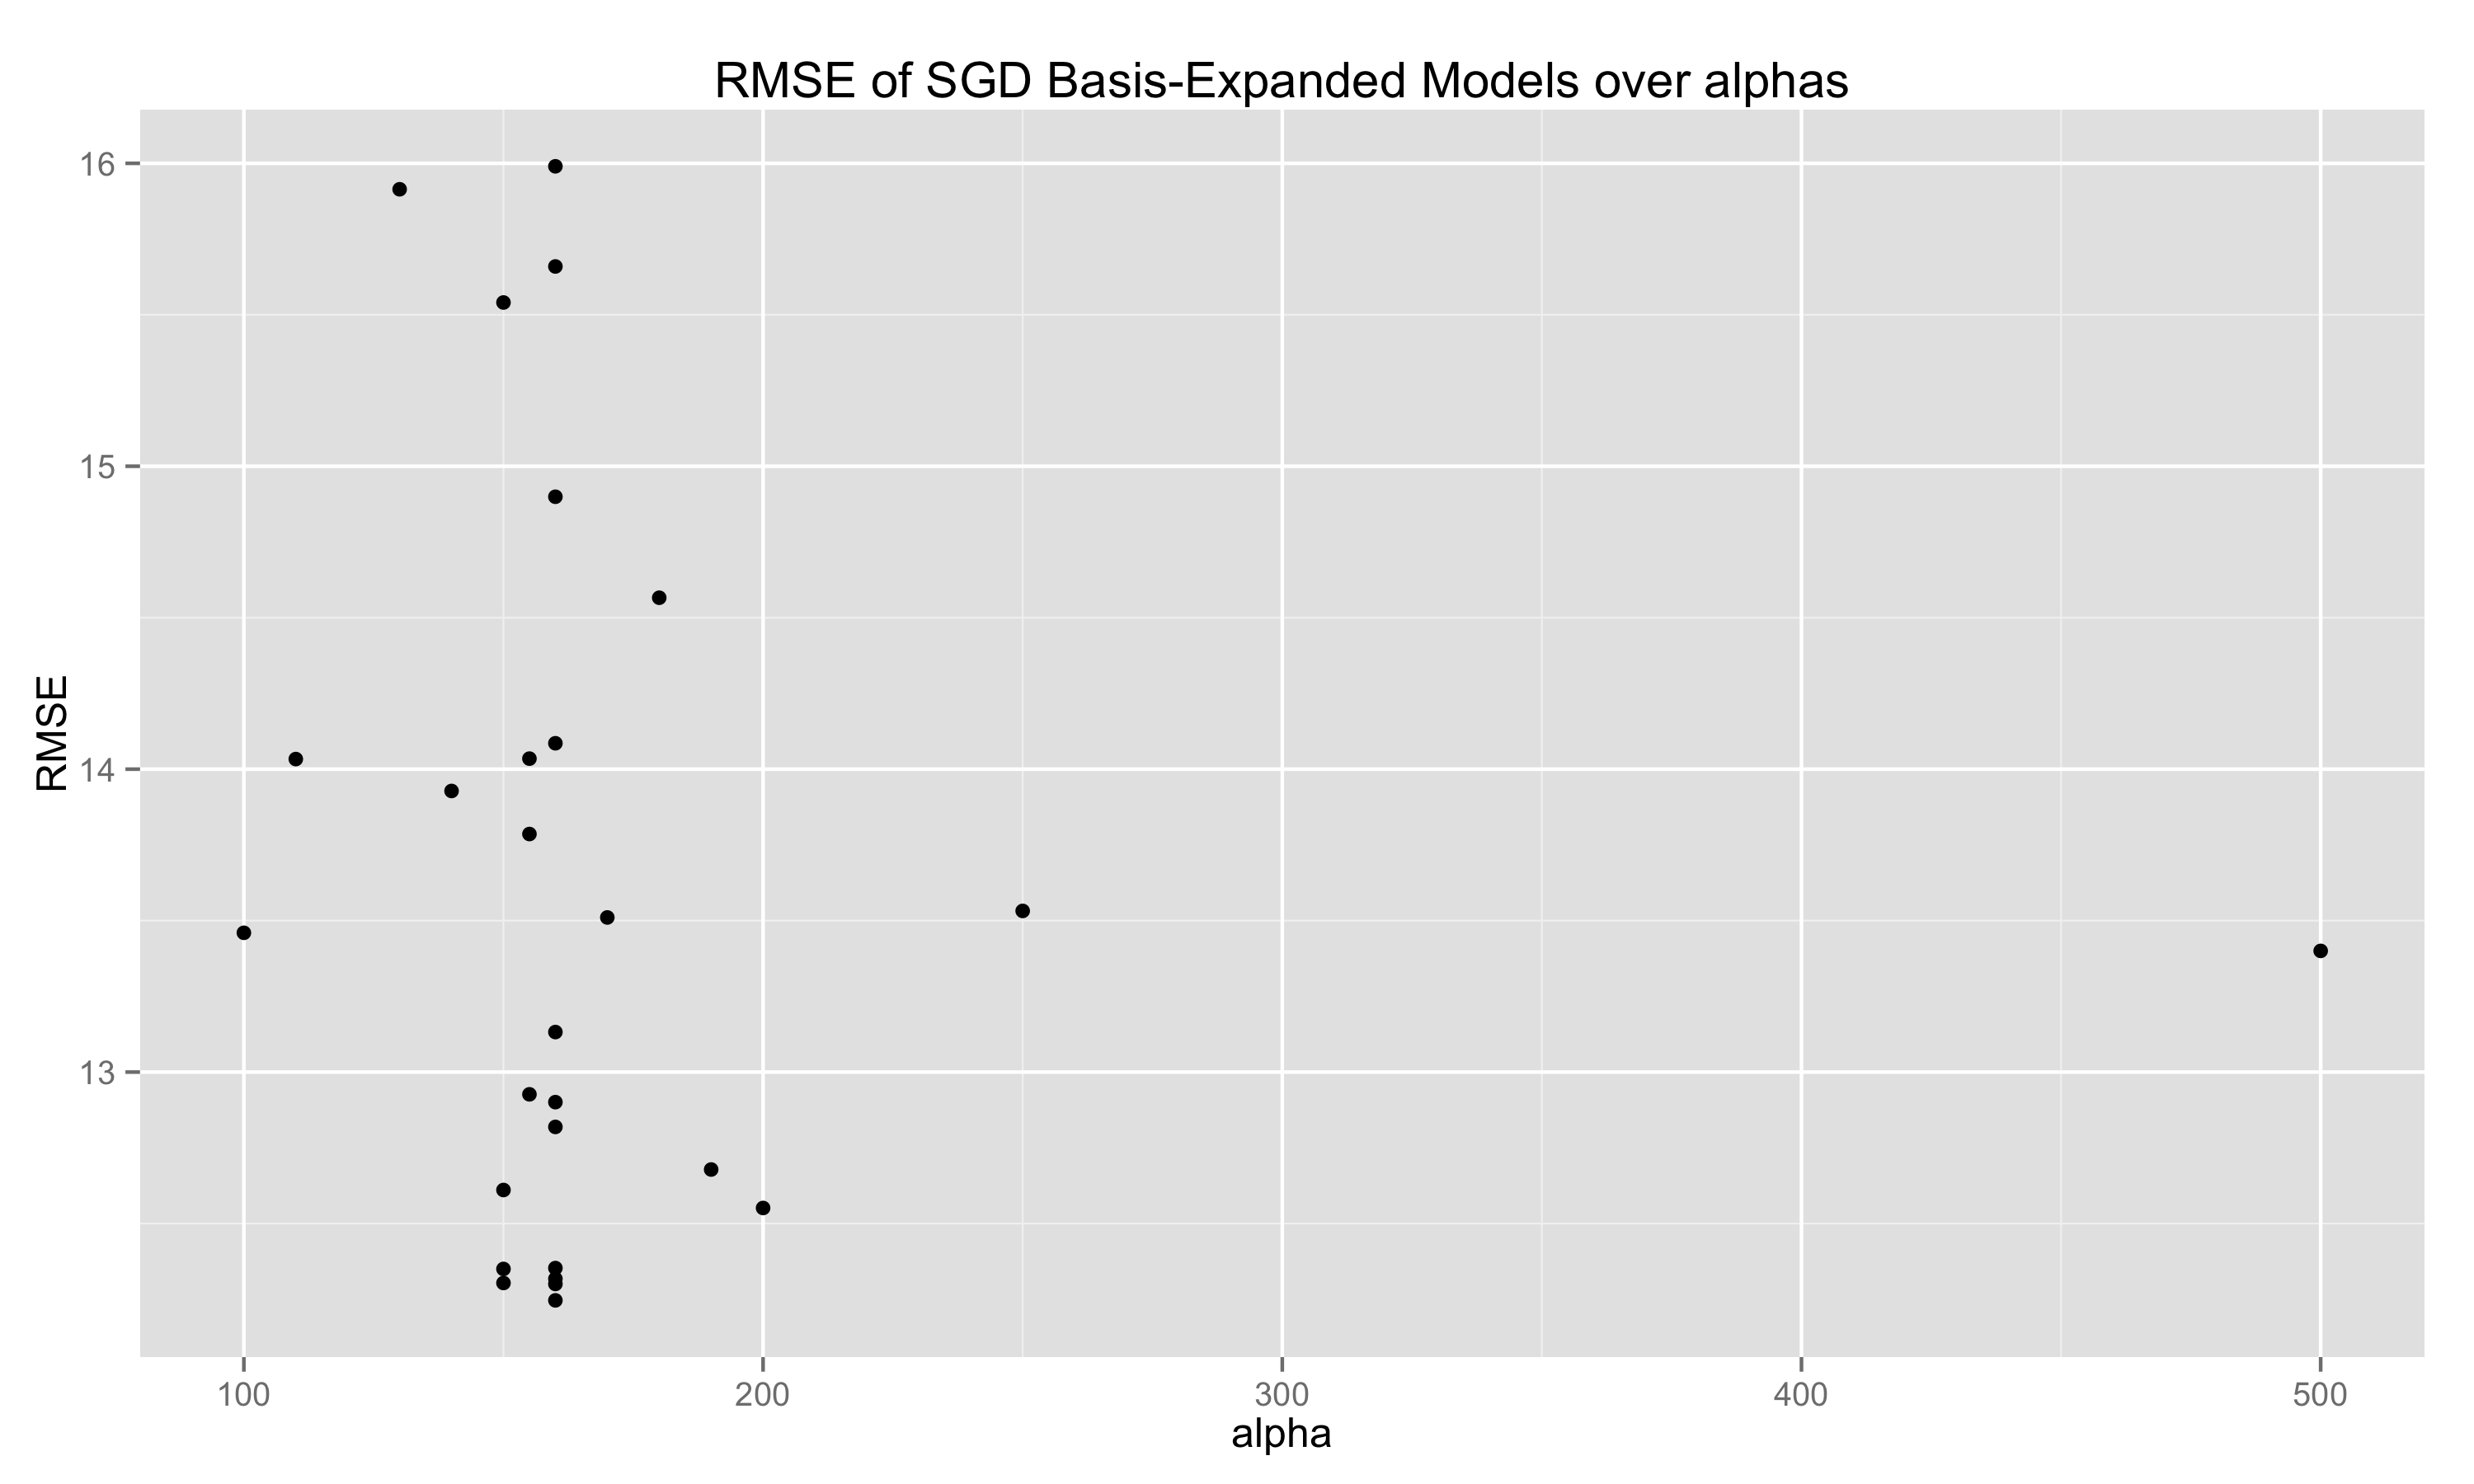
\includegraphics[width=140mm]{figs/basis_expand_RMSE_alpha.png}
\caption{Many different values of $\alpha$ are used for fitting the basis-expanded model during SGD, but none of the resulting models achieve an RMSE lower than the highest-performing linear models.  Moreover, different iterations of a model trained using a given $\alpha$ (for example, $\alpha = 160$) give largely variable RMSE scores.}
\label{fig:basis_results}
\end{figure}
\begin{figure}
\centering
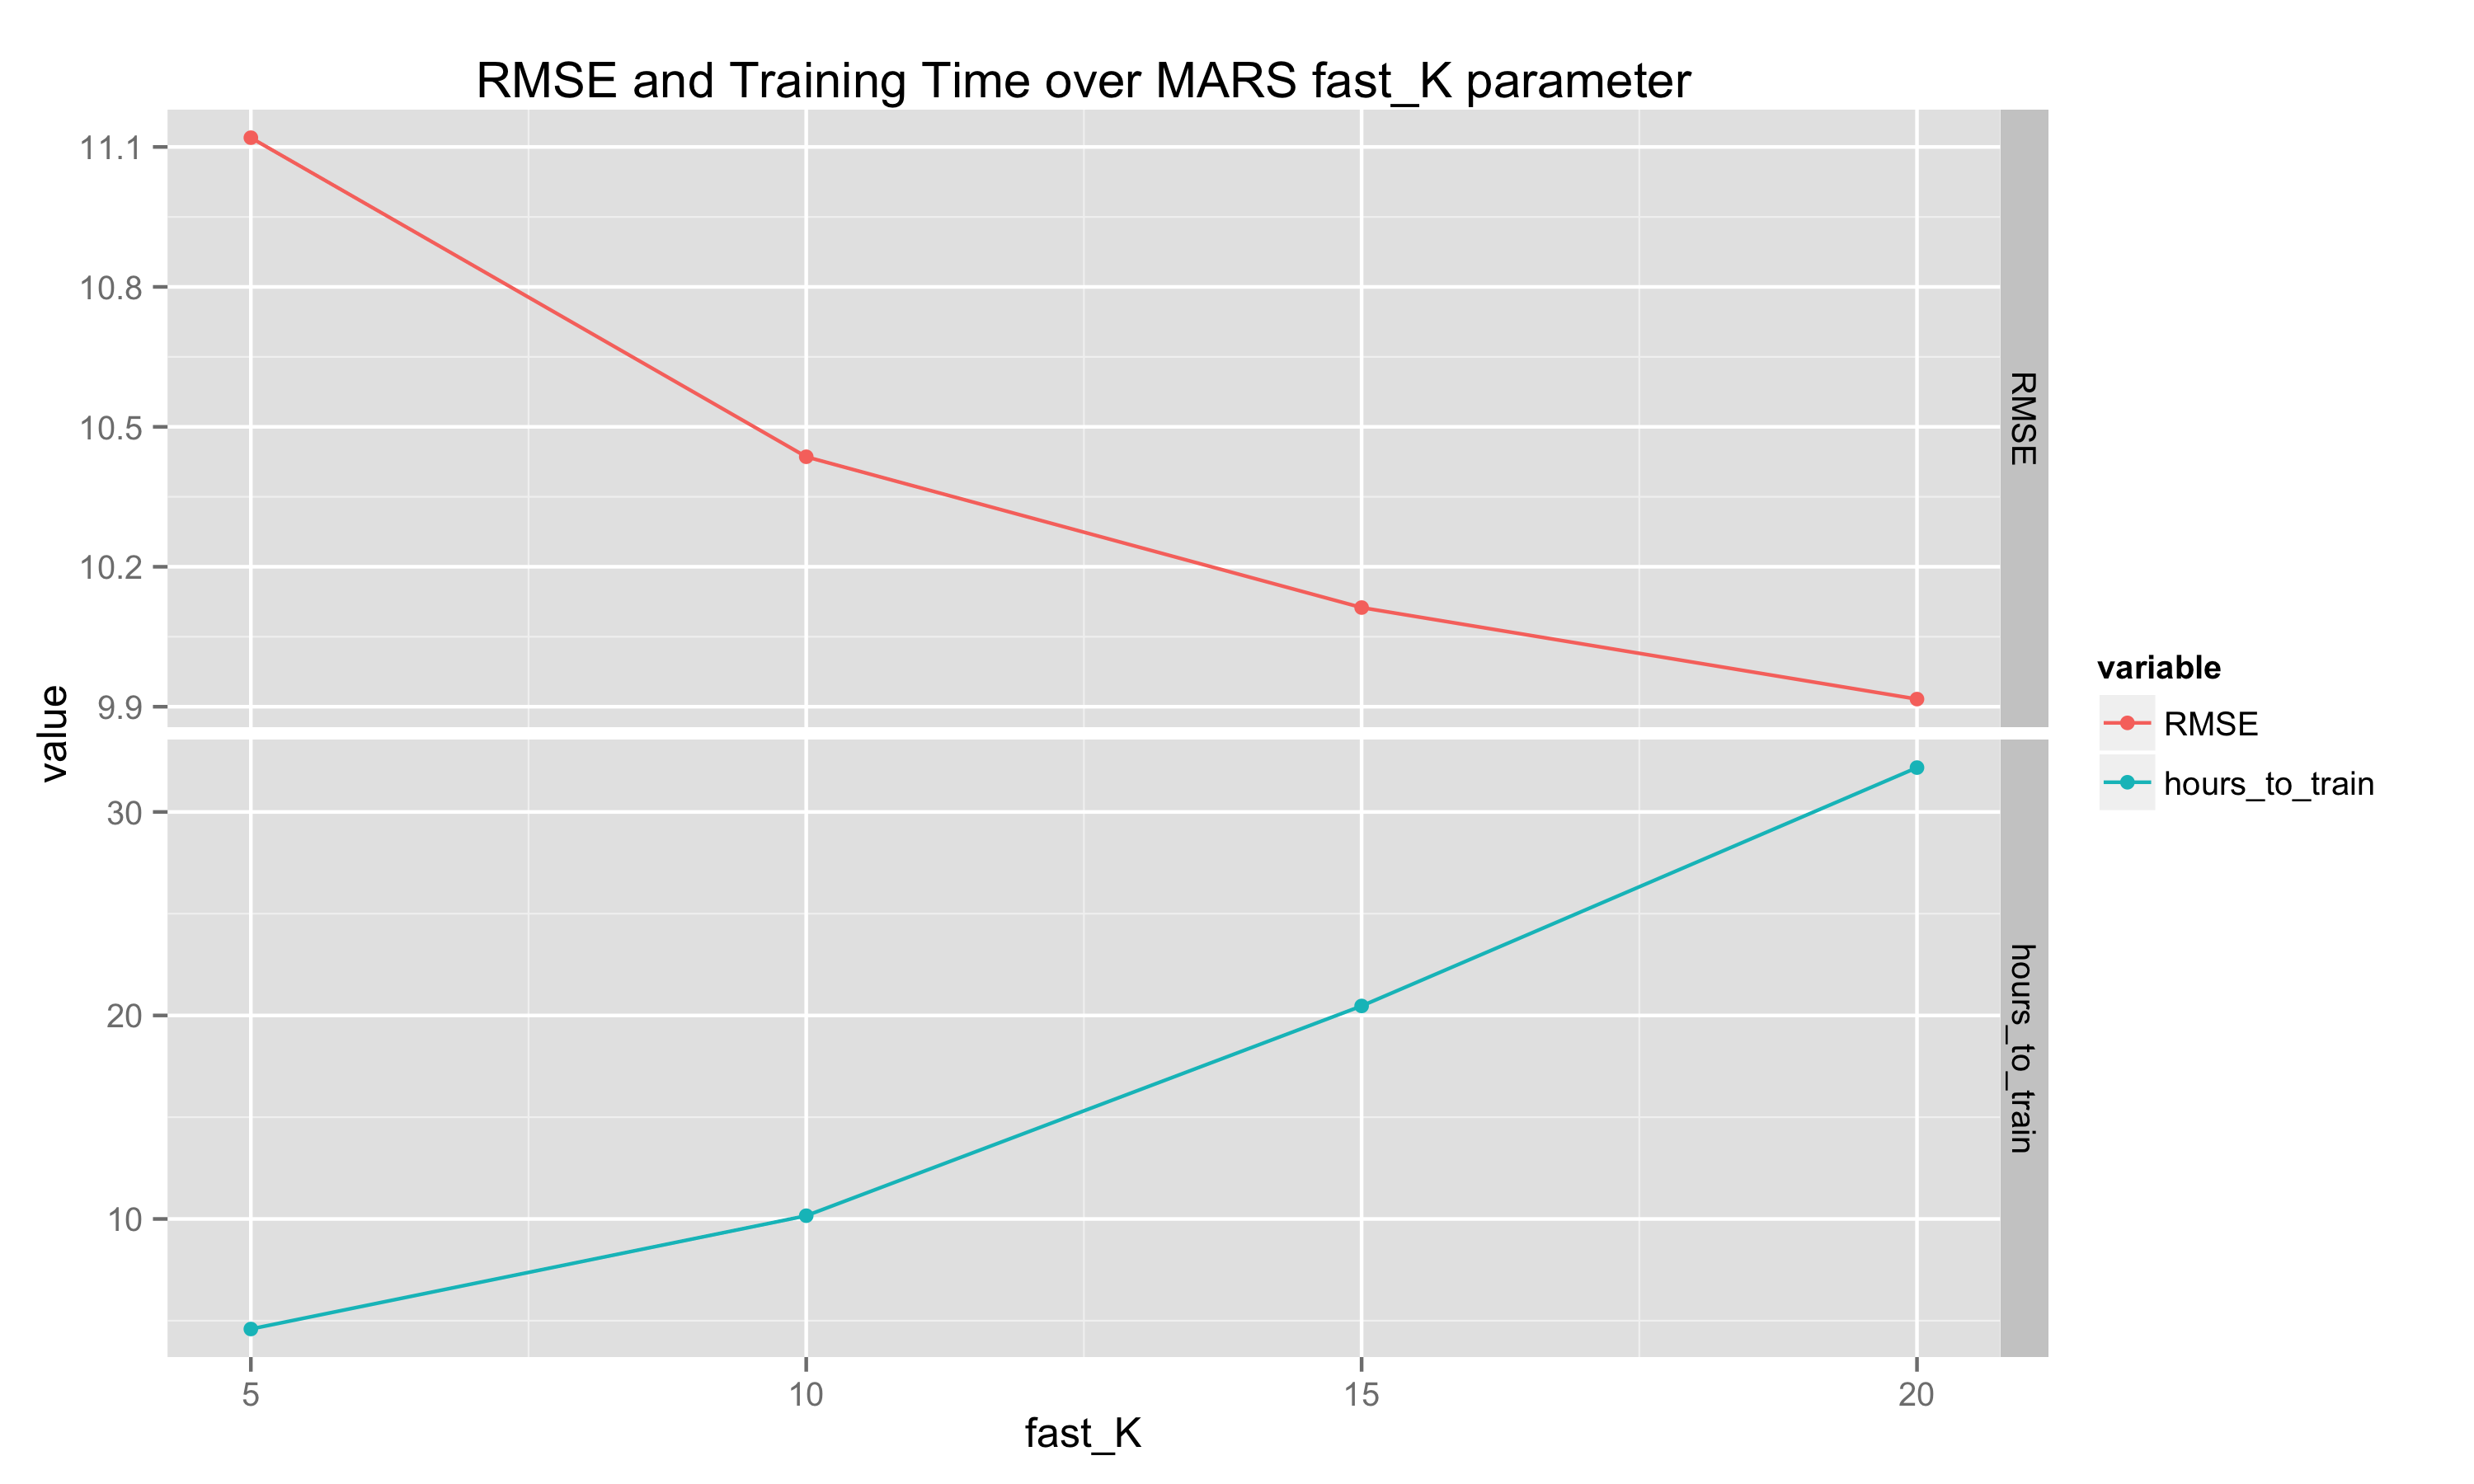
\includegraphics[width=155mm]{figs/mars_rmse.png}
\caption{RMSE and training time of MARS models for various values of ``fast K''.  Even the lowest values of ``fast K'' result in RMSE lower than the linear and basis-expanded models, while increasing ``fast K'' brings an even more drastic decrease (albeit at the expense of longer training times).}
\label{fig:mars_rmse}
\end{figure}
\clearpage
\section{Discussion}\label{sec:discussion}
Our original goal was to answer three questions, which largely relied on each other in succession.  First, for the problem of applying the direct perception paradigm for autonomous driving, we asked if immediately historical data is predictively useful.  We provided an unequivocally positive answer to this question by using ordinary least squares to fit simple and interpretable models for two models: Model 1, which used 500 convoluted image features for the current time step $t$, and Model 2, which used the 500 convoluted image features from the $t-1$ step alongside the current 500 features.  We saw that the distribution of the p-values for the coefficients corresponding to the $t-1$ features in Model 2 pointed to a very high significance level, one that completely confirms the importance of history.\par
Our second question, conditional upon a positive answer to the first, delved deeper -- we sought to rigorously determine not just if, but how much history was predictively relevant.  We answered this question by using stochastic gradient descent to fit a set of models that included incrementally more steps of history, and comparing the subsequent stacked information criterion metrics.  This process showed that for our TORCS data, including the most recent 7 data points gave the best performance with respect to prediction for the validation set.\par
Finally, we simply wanted to validate that applying more complex, nonlinear models on data that included history would improve upon the predictive power of our linear recurrent models.  We fit both basis-expanded and MARS models, and found that the MARS models, which employ a similar iterative forward-backward training process to neural networks, achieved a performance significantly better than our linear recurrent models.\par
We were able to thoroughly answer all three of our questions with rigorous statistical analysis.  Note that we do not seek to compare our highest-performing nonlinear model to \cite{deepdriving} on a performance basis.  The goal for this paper was to establish confirmation of the importance and feasibility of using history and recurrency in the TORCS driving problem.  Therefore, a next extension of both this work and the work of \cite{deepdriving} would make use of more advanced and powerful models as \cite{deepdriving} did, but also factor a recurrence in.  This could be done either through training a state-of-the-art non-recurrent model on recurrent data, similar to our methodology (for example, applying a convolutional neural network to recurrent data), or through using an actual recurrent model (a recurrent neural network, or more specifically, a Long Short-Term Memory neural network, applied to the non-recurrent data).
\end{document} 
